%% Define title of slide deck

\newcommand\CourseTopic{Motivation}
\newcommand\CourseTopicShort{Motivation}
\newcommand\CourseNumber{1}

\newcommand\CourseDate{\today}
\newcommand\CourseInstitute{ETH Zurich}
\newcommand\CourseAbbreviation{OR}
\newcommand\CourseTitle{Operations Research in R}
\newcommand\CourseAuthor{Stefan Feuerriegel}

\newcommand{\CourseQuiz}{Visit webpage with course quiz.}
\newif\ifQuizSolution\QuizSolutionfalse

\PassOptionsToPackage{table,dvipsnames}{xcolor}
\documentclass[%
  final,
  11pt, 
  show notes, % enables Notes
  t, % Place text of slides at the (vertical) top of the slides
  fleqn, % equations are centered
]{beamer} 

\usepackage{booktabs}

\newcommand\const{\mathsf{const.}}
\newcommand\rp{^{-1}}
\newcommand\rps{^{-2}}
\newcommand\rpc{^{-3}}

\newcommand\transpose{^T} %{^\top}
\newcommand\rptranspose{^{-T}} %^{^{-\top}}
\newcommand\pseudoinverse{^{+}}

\newcommand\define{:=} % :=, \ensuremath{\mathrel{\stackrel{\mathsf{def}}{=}}}
\newcommand\ldefine{=:}
\newcommand{\setsep}{\, | \,}

\newcommand{\correspond}{\mathrel{\widehat{=}}}

\newcommand{\norm}[1]{\left\Vert #1 \right\Vert}
\newcommand{\floor}[1]{\left\lfloor #1 \right\rfloor}
\newcommand{\ceil}[1]{\left\lceil #1 \right\rceil}

\newcommand{\vecval}[1]{\bm{#1}}
\newcommand{\matval}[1]{#1}

\newcommand{\sspace}{\quad}
\newcommand{\wspace}{\qquad}

\newcommand{\sand}{\sspace\text{and}\sspace}
\newcommand{\wand}{\wspace\text{and}\wspace}
\newcommand{\for}{\text{for }}

\newcommand{\R}{\mathbb{R}}
\newcommand{\N}{\mathbb{N}}

\newcommand{\unitvec}[2]{{\vecval{u}_{#1}}}
\newcommand{\identitymat}[1]{\matval{\mathup{I}}_{#1,#1}}
\newcommand{\permutemat}{\matval{\Pi}}
\newcommand{\zerovec}[1]{\vecval{0}_{#1}}
\newcommand{\zeromat}[2]{\matval{0}_{#1,#2}}

\newcommand{\fulfill}{\stackrel{!}{=}}
\newcommand{\inlineortho}{\bot}
\newcommand{\ortho}{\,\, \inlineortho \,\,}
\newcommand{\iszero}[1]{\underbrace{#1}_{=0}}

\newcommand{\vecsize}[1]{\in\R^{#1}}
\newcommand{\matsize}[2]{\in\R^{#1 \times #2}}

\newcommand{\concatmat}[1]{\Concat{#1}}
\newcommand{\concatvec}[1]{\left[#1\right]}
\newcommand{\concatmatsep}{\, | \,}
%\newcommand{\lincomb}[1]{\left\langle #1 \right\rangle}
\newcommand{\lincomb}[1]{\linearspan{#1}}
%\newcommand{\vecprod}[2]{\left( #1, #2 \right)}
\newcommand{\vecprod}[2]{\left\langle #1, #2 \right\rangle}

\newcommand{\abs}[1]{\left\lvert #1 \right\rvert}
\newcommand{\sign}[1]{\mathup{sign}\left( #1 \right)}
%\newcommand{\ssign}{\mathsf{sign}}
\newcommand{\diag}{\operatorname{diag}}
%\renewcommand\Re[1][]{\mathsf{Re}\,#1}
%\renewcommand\Im[1][]{\mathsf{Im}\,#1}

\newcommand{\vvector}[2]{\left[\begin{array}{c} #1 \\ #2 \end{array} \right]}
\newcommand{\vvvector}[3]{\left[\begin{array}{c} #1 \\ #2 \\ #3 \end{array} \right]}

\newcommand{\intervaloo}[2]{\left(#1,#2\right)}
\newcommand{\intervaloc}[2]{\left(#1,#2\right]}
\newcommand{\intervalco}[2]{\left[#1,#2\right)}
\newcommand{\intervalcc}[2]{\left[#1,#2\right]}

\newenvironment{mmatrix}{\begin{bmatrix}}{\end{bmatrix}}

\newcommand{\Oh}[1]{\mathsf{O}\left(#1\right)}

\newcommand{\e}[1]{\mathup{e}^{#1}}

\newcommand{\dd}{\mathop{}\!\mathsf{d}}
\newcommand{\Laplace}{\Updelta}

\newcommand\op[1]{{\hat{\mathsf{#1}}}}  % Operator

\newcommand\imaginary{\mathup{i}}

% use together with long limits in \sum, \prod, etc
% from mathmode, p. 63
  \def\clap#1{\hbox to 0pt{\hss#1\hss}}
  \def\mathclap{\mathpalette\mathclapinternal}
  \def\mathclapinternal#1#2{%
    \clap{$\mathsurround=0pt#1{#2}$}
  }

\newcommand\ie{i.\,e.\xspace}
\newcommand\eg{e.\,g.\xspace}
\newcommand\etc{etc.\xspace}
\newcommand\cf{cf.\xspace}

%% from: http://tex.stackexchange.com/questions/2441/how-to-add-a-forced-line-break-inside-a-table-cell
\newcommand{\mcell}[2][c]{%
  \begin{tabular}[c]{@{}#1@{}}#2\end{tabular}}
\newcommand{\mcellt}[2][c]{%
  \begin{tabular}[t]{@{}#1@{}}#2\end{tabular}}

\newcommand{\stackedcell}[2][c]{%
  \begin{tabular}[#1]{@{}c@{}}#2\end{tabular}}

<<setup, include=FALSE>>=
# change default language to display error messages in English
Sys.setenv(LANGUAGE = "en")

# smaller font size for chunks
library(knitr)
opts_chunk$set(size = "footnotesize", fig.width = 3, fig.height = 3)
@

\begin{document}

  \begin{frame}%[plain]
  \titlepage
\end{frame}
  % \section[Contents]{}

\begin{frame}<beamer>%[allowframebreaks]
  \frametitle{Outline}
  \tableofcontents[%
%     currentsection, % causes all sections but the current to be shown in a semi-transparent way.
%     currentsubsection, % causes all subsections but the current subsection in the current section to ...
%     hideallsubsections, % causes all subsections to be hidden.
%     hideothersubsections, % causes the subsections of sections other than the current one to be hidden.
%     part=, % part number causes the table of contents of part part number to be shown
%    pausesections, % causes a \pause command to be issued before each section. This is useful if you
%     pausesubsections, %  causes a \pause command to be issued before each subsection.
%     sections={ overlay specification },
%      sectionstyle=show/shaded,
      subsectionstyle=hide
  ]
\end{frame}
  
\section{Introduction to Optimization}

\begin{frame}[fragile]
  \frametitle{Mathematical Optimization}
\begin{itemize}
\item Optimization uses a rigorous \emph{mathematical model} to determine the most efficient solution to a described problem 
\item One must first identify an \emph{objective}
\begin{itemize}
\item Objective is a quantitative measure of the performance
\item Examples: profit, time, cost, potential energy
\item In general, any quantity (or combination thereof) represented as a \emph{single number}
\end{itemize}
\end{itemize}
\begin{center}
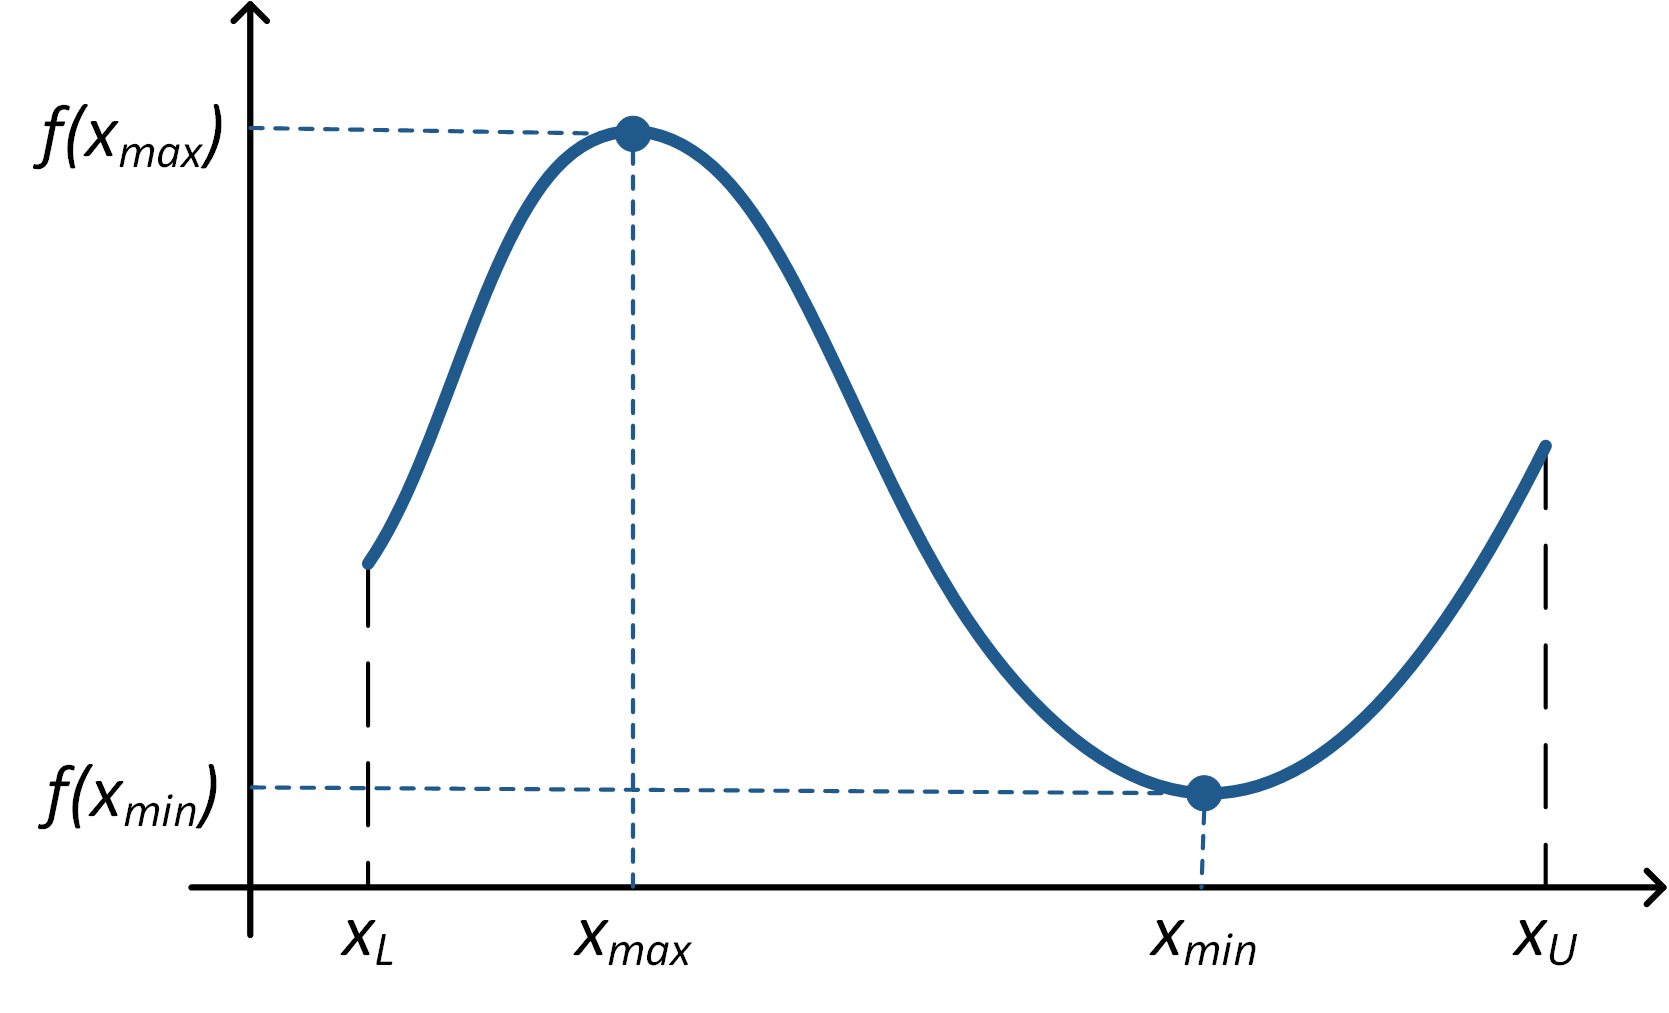
\includegraphics[width=.55\textwidth]{extreme_value_theorem}
\end{center}
\end{frame}

\begin{frame}[fragile]
  \frametitle{Applications of Optimization}
%Optimization is used \emph{in many ares} of business and economics, e.\,g.:
\begin{itemize}
\item \emph{Management} 
\begin{itemize}
\item Determining product portfolios
\item Location planning
\item Investments decisions
\end{itemize}
\item \emph{Game theory} 
\begin{itemize}
\item Comparing players' strategies
\end{itemize}
\item \emph{Logistics} 
\begin{itemize}
\item Finding optimal routes and schedules
\end{itemize}
\item \emph{Design decisions} 
\begin{itemize}
\item Constructing processes, plants and other equipment
\end{itemize}
\item \emph{Operation} 
\begin{itemize}
\item Adjustment to changes in environmental conditions, production planning, control, etc.
\end{itemize}
\item \emph{Mathematical modeling} 
\begin{itemize}
\item Parameter estimation
\item Model discrimination
\end{itemize} 
\end{itemize}
\end{frame}

\begin{frame}[fragile]
  \frametitle{Optimization Problem}
Optimization is the \emph{minimization or maximization} of a function \\
subject to (s.\,t.) constraints on its variables

\vspace*{0.4cm}
\textbf{Notation:} General form
\begin{align*}
\min\limits_{\vecval{x}} f(\vecval{x}) \quad\text{s.\,t.}\quad & h(\vecval{x}) = 0 \\
 & g(\vecval{x}) \leq 0
\end{align*}
with
\begin{itemize}
\item $\vecval{x} \in\R^n$ as the \emph{variable}, \emph{unknown} or \emph{parameter}
\item \emph{Objective function} $f : D \rightarrow \R$, $D \subseteq \R^n$
\item \emph{Equality constraints} $h : D_h \rightarrow \R^l$, $D_h \subseteq \R^n$
\item \emph{Inequality constraints} $g : D_g \rightarrow \R^k$, $D_g \subseteq \R^n$
\end{itemize}
\end{frame}

\begin{frame}[fragile]
  \frametitle{Properties of Optimization Problems}
{\renewcommand{\arraystretch}{1.8}%
\begin{tabular}{ll}
\textbf{Objective} & Linear, quadratic, non-linear, etc. \\
\textbf{Constraints} & Equality and inequality \\
\textbf{Variable types} & $\vecval{x}$ can be continuous, integer, mixed \\
\textbf{Direction} & $\min\limits_{\vecval{x}} f(\vecval{x}) \Leftrightarrow \max\limits_{\vecval{x}} -f(\vecval{x})$ \\
\textbf{Bounds} & Lower $\vecval{x}_L \leq \vecval{x}$ or upper $\vecval{x} \leq \vecval{x}_U$ \\
\textbf{Dimension} & One dimensional if $n = 1$, or multi-dimensional if $n > 1$ \\
\textbf{Optima} & Isolated, local or global nature \\
\end{tabular}
}
\end{frame}

\begin{frame}[fragile]
  \frametitle{Classification of Optimization Problems}
\begin{itemize}
\item \emph{Linear Programming (LP)} 
\begin{itemize}
\item Objective function and constraints are linear
\item $\min\limits_{\vecval{x}} \vecval{c}^T \vecval{x}$ s.\,t. $A \vecval{x} \leq \vecval{b}$, $\vecval{x} \geq 0$
\end{itemize}
\item \emph{Quadratic Programming (QP)} 
\begin{itemize}
\item Objective function is quadratic and constraints are linear
\item $\min\limits_{\vecval{x}} \vecval{x}^T Q \vecval{x}$ s.\,t. $A \vecval{x} \leq \vecval{b}$, $\vecval{x} \geq 0$
\end{itemize}
\vspace*{0.4cm}
\item \emph{Non-Linear Programming (NLP):} objective function or at least one constraint is non-linear
\vspace*{0.4cm}
\item \emph{Integer Programming (IP):} all variables are discrete
\item \emph{Mixed Integer Programming (MIP)} 
\begin{itemize}
\item Continuous and discrete variables
\item Problem can be linear (MILP) or non-linear (MINLP)
\end{itemize}
\end{itemize}
\end{frame}

\begin{frame}[fragile]
  \frametitle{Classification of Optimization Problems}
\begin{itemize}
\item \emph{Dynamic Optimization:} solution is a function of time
\item \emph{Stochastic Optimization}
\begin{itemize}
\item Model cannot be fully specified, but has uncertainties with confidence estimates
\item Optimize expected performance given uncertainty
\end{itemize}
\end{itemize}

\begin{exampleblock}{Question}
\begin{itemize}
\item What type is the following optimization problem?
\begin{equation*}
\max\limits_{x,y} 3x + y^2
\quad
\text{s.\,t.}
\quad 
x + y < 10 \text{ and } y \in \left\{ 1, 2, 4, 8 \right\}
\end{equation*}
\begin{itemize}
\item MIP
\item MILP
\item MINLP
\end{itemize}
\item \CourseQuiz
\end{itemize}
\end{exampleblock}
\end{frame}

\begin{frame}[fragile]
  \frametitle{Optimal Solution}
\begin{itemize}
\item $x^\ast$ is a \emph{global minimum} if $x^\ast \in D$ and
\begin{equation*}
f(x^\ast) \leq f(x) \qquad \text{for all } x \in D
\end{equation*}
\end{itemize}

\begin{columns}[T]
\begin{column}{.65\textwidth}
$\rightarrow$ Global minimizers are desired, though often one has only local knowledge of $f$
\end{column}
\begin{column}{.3\textwidth}
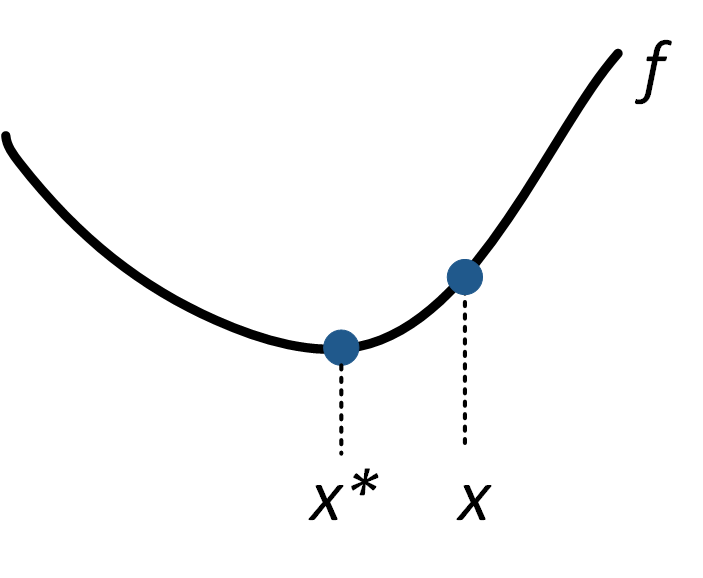
\includegraphics[width=\textwidth]{optimization_problem}
\end{column}
\end{columns}
\end{frame}

\begin{frame}[fragile]
  \frametitle{Optimal Solution}
Examples of optimal solutions:

\vspace*{0.4cm}
% copy visualizations from ANOR_L1/slide 33
\begin{tabular}{cc}
Isolated global solution & One global, two local solutions \\
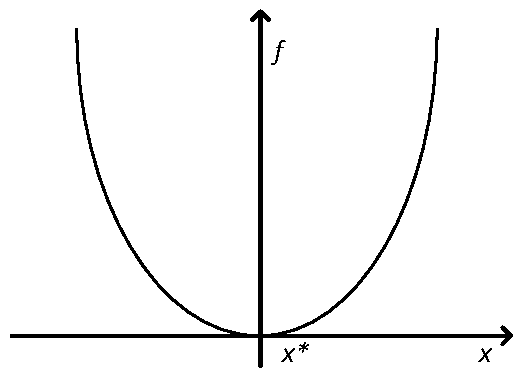
\includegraphics[width=.3\textwidth]{isolated_global_solution} & 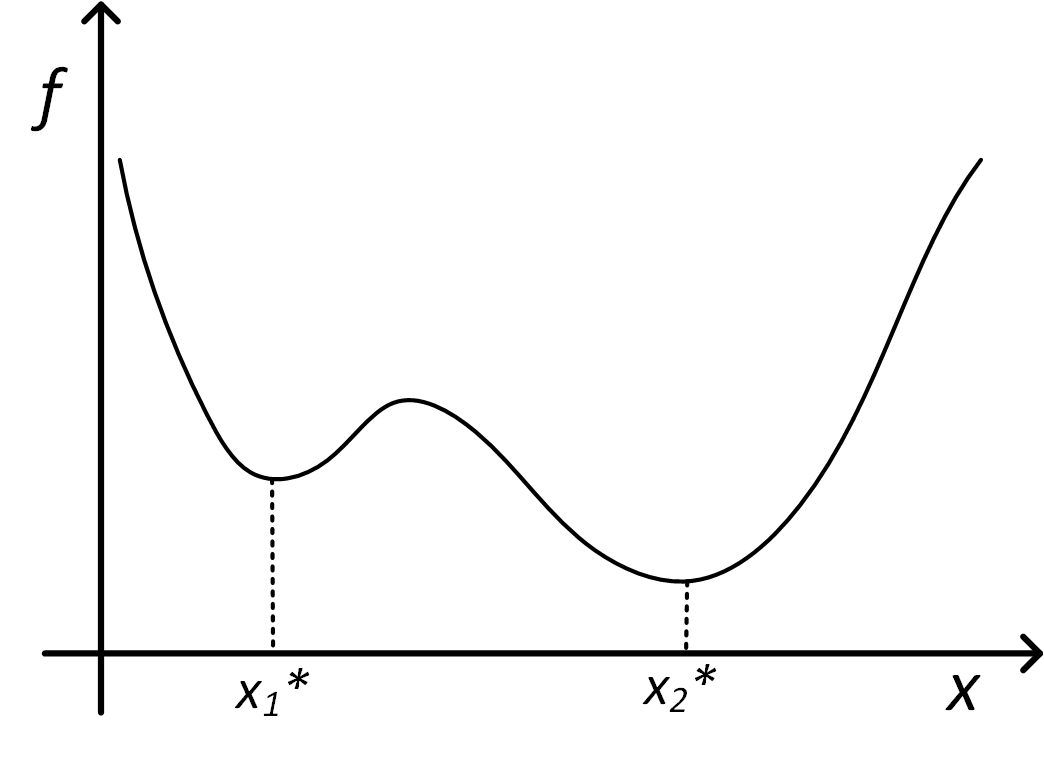
\includegraphics[width=.3\textwidth]{two_local_solutions} \\
A local but no global solution & Many non-isolated, global solutions \\
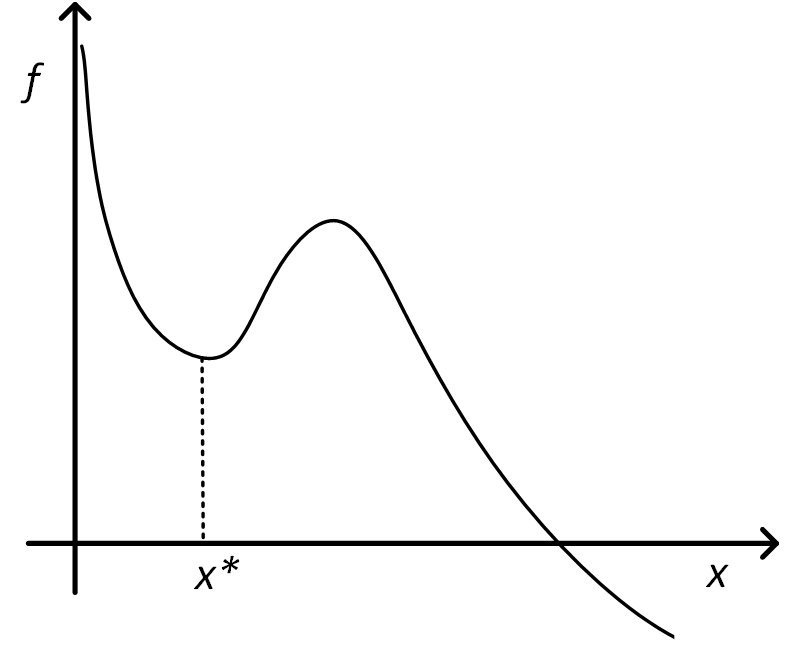
\includegraphics[width=.3\textwidth]{local_non-global_solution} & 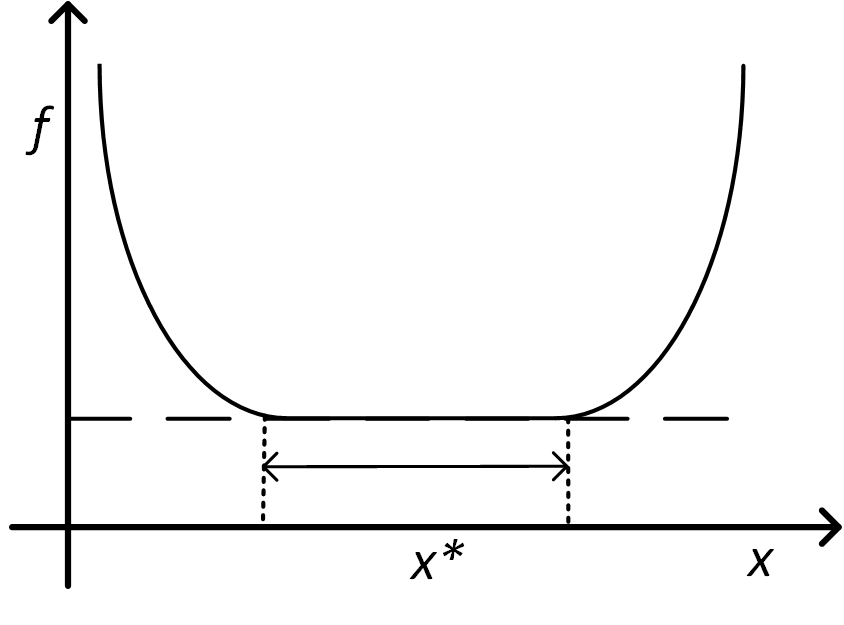
\includegraphics[width=.3\textwidth]{non-isolated_global_solution}
\end{tabular}
\end{frame}

\begin{frame}[fragile]
  \frametitle{Optimization Procedure}
\emph{Formulation and solution} of optimization problems usually follows:
\begin{enumerate}
\item \emph{Analysis of environment} to determine the variables of interest
\item Definition of optimality criteria as an \emph{objective function} with (additional) constraints
\item Formulation as a \emph{mathematical model} with degrees of freedom
\item \emph{Numerical optimization} to find a solution
\item \emph{Verification of the solution} through sensitivity analysis (with respect to the assumptions made in the problem formulation)
\end{enumerate}
\end{frame}

\section{Motivation}

% TODO
%\begin{frame}[fragile]
%  \frametitle{Profit Maximization}
%\begin{itemize}
%\item % see seminar paper
%\end{itemize}
%\end{frame}

% TODO
%\begin{frame}[fragile]
%  \frametitle{Allocation}
%\begin{itemize}
%\item % LP
%\end{itemize}
%\end{frame}

\begin{frame}[fragile]
  \frametitle{Production Scheduling}
\textbf{Problem}
\begin{itemize}
\item Given plants $i = 1, \ldots, M$ where each \emph{manufactures} $P_i$ goods
\item Each plant has a \emph{maximal output} $O_i$
\item Each plant manufactures at a \emph{capacity-specific cost} $C_i(P_i)$, which gives the cost as a function of the production
\item Each customer $j = 1, \ldots, N$ \emph{requests} $C_j$ goods
\end{itemize}

\vspace*{0.2cm}
\textbf{Objective function}: find the \emph{optimal production schedule} such that the manufacturing and shipment costs are minimized

\begin{center}
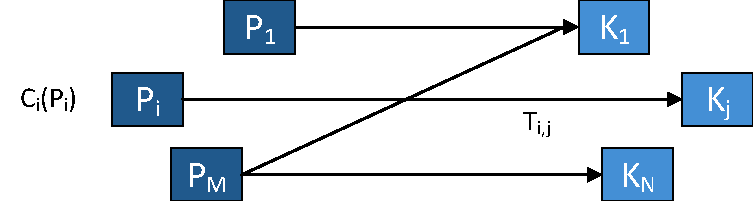
\includegraphics[width=.8\textwidth]{problem_product_scheduling}
\end{center}
\end{frame}

\begin{frame}[fragile]
  \frametitle{Portfolio Optimization}
\textbf{Problem}
\begin{itemize}
\item Investor wants to \emph{invest} money such that it \emph{maximizes the investor's utility}
\item Utility $U$ depends on \emph{daily return} $\mu$ and \emph{risk} $\sigma^2$
\item Given risk taking $\kappa$, then $U(\mu, \sigma^2) = \mu - \frac{\kappa}{2} \sigma^2$
\end{itemize}

\vspace*{0.2cm}
\textbf{Objective function}: \emph{Maximize $U(\mu, \sigma^2)$} among a range of stocks $s_1, \ldots s_N$
\vspace*{0.2cm}

\begin{columns}[T]
\begin{column}{.4\textwidth}
\hspace{1cm}
%{\footnotesize
\begin{tabular}{c ccc}
$\vecval{c}^T$ & $s_1$ & $s_2$ & $s_3$ \\
\midrule
$\mu$ & 0.2 & 0.5 & 0.1
\end{tabular}
%}
\end{column}
\begin{column}{.65\textwidth}
\hspace{1cm}
%{\footnotesize
\begin{tabular}{c ccc}
$Q$ & $s_1$ & $s_2$ & $s_3$ \\
\midrule
$s_1$ & 0.1 & 0.02 & 0.02 \\
$s_2$ & 0.02 & 0.1 & 0.02 \\
$s_3$ & 0.02 & 0.02 & 0.1
\end{tabular}
%}
\end{column}
\end{columns}
\begin{equation*}
\Rightarrow
\max\limits_{\vecval{x}} \vecval{c}^T \vecval{x} - \frac{\kappa}{2} \vecval{x}^T Q \vecval{x}
\quad
\text{s.\,t.}
\quad
x_i \geq 0 \text{ and } \sum\limits_i{x_i} = 1
\end{equation*}
\end{frame}

\begin{frame}[fragile]
  \frametitle{Portfolio Optimization in R}
<<quadprog,eval=FALSE>>=
library(quadprog) # load necessary library
@
<<,include=FALSE>>=
<<quadprog>>
@
\vspace*{-0.6cm}
<<>>=
kappa <- 4 # set risk taking
# objective function
c <- c(0.02, 0.05, 0.01)
Q <- matrix(c(0.1,0.02,0.02, 0.02,0.1,0.02, 
              0.02,0.02,0.1), nrow=3)
# constraints
A <- matrix(c(1,1,0,0, 1,0,1,0, 1,0,0,1), nrow=4)
b <- c(1, 0, 0, 0)

sol <- solve.QP(kappa/2*Q, c, t(A), b, meq=1) # call solver
sol$solution # ratio of stocks in portfolio
sol$value # minimum value of objective function
@
\end{frame}

\begin{frame}
  \frametitle{Outlook}
\begin{enumerate}
\item \emph{Introduction to R}
\item \emph{Advanced R} 
\begin{itemize}
\item Programming prerequisites 
\item Visualize optimization routines
\end{itemize}
\item \emph{Numerical Analysis:} 
\begin{itemize}
\item Mathematical prerequisites to derive and formalize optimization routines
\end{itemize}
\item \emph{Optimization in R:}
\begin{itemize} 
\item Use of built-in optimization routines
\end{itemize}
\end{enumerate}
\end{frame}

\end{document}

